\documentclass[11pt]{article}

\usepackage[margin=1in]{geometry}
\usepackage{graphicx}
\usepackage{booktabs}
\usepackage{xcolor}
\usepackage{listings}
\usepackage[hidelinks]{hyperref}
\usepackage{parskip}
\usepackage{enumitem}
\usepackage{titlesec}

\graphicspath{{figures/}}
\setlist[itemize]{leftmargin=1.4em, itemsep=2pt, topsep=3pt}

% tighter, report-style section headings (not paper-style)
\titleformat{\section}{\large\bfseries}{}{0pt}{}
\titlespacing{\section}{0pt}{14pt}{4pt}
\titleformat{\subsection}{\normalsize\bfseries}{}{0pt}{}
\titlespacing{\subsection}{0pt}{10pt}{2pt}

\definecolor{promptbg}{HTML}{F7F5F2}
\definecolor{tldrbg}{HTML}{EEF4FA}
\definecolor{muted}{HTML}{69757F}
\lstset{
  basicstyle=\ttfamily\footnotesize, breaklines=true, breakindent=0pt,
  columns=fullflexible, backgroundcolor=\color{promptbg}, frame=single,
  rulecolor=\color{lightgray}, xleftmargin=4pt, xrightmargin=4pt, aboveskip=6pt, belowskip=10pt,
}

\begin{document}

\pagestyle{empty}

{\LARGE\bfseries Adaptive Test-Ordering with an LLM}\\[4pt]
{\color{muted} Weekly update \textbullet\ 2026-07-17}

\medskip
\noindent\fcolorbox{gray!35}{tldrbg}{\parbox{0.97\linewidth}{\small
\textbf{TL;DR.} On MIMIC, the strictest prompt reaches the same ordering concordance as the plain prompt while ordering about 30\% fewer tests at about 40\% lower cost, and it orders fewer tests than the clinicians actually did. On CPC, diagnostic accuracy stays high (78--86\%) while the strict prompt more than halves the test count. Both results reproduce in a second independent sweep. Two environment problems (a MIMIC gatekeeper that fabricates most results, and a CPC comparison against the entire published record) mean the model-versus-human head-to-head is not reported as a result; the efficiency claim rests on accuracy and concordance paired with cost.}}

\section{Progress this week}
\begin{itemize}
\item Split generation from evaluation, so transcripts are saved once and metrics re-score off them for free.
\item Made concordance and harm deterministic (no LLM), so they are reproducible and cost nothing to compute.
\item Added precision alongside recall, which is where the prompts actually separate; recall alone rewards over-ordering.
\item Added experiment tracking: every run carries the config and the exact prompt text that produced it, and a second tagged sweep reproduces the first within confidence intervals.
\item Found and fixed two truncation bugs (gatekeeper panels, CPC extractor) by reading the transcripts, which is also how the two limitations below turned up.
\end{itemize}

\section{Methods}

\textbf{Task and agents.} Each case runs as a sequential diagnosis with three agents. The \emph{gatekeeper} holds the full case, including the true diagnosis, and answers one request at a time: it gives the presentation, then returns the finding for each specific test that is ordered. The \emph{recommender} reads the presentation and orders tests through the gatekeeper in one running conversation, using each result to decide what to order next, and stops when the work-up is complete. The \emph{judge} scores the final diagnosis. All prompts are in the appendix.

\textbf{Case sources.} CPC: 50 NEJM clinicopathological conference cases, each a narrative vignette with a known diagnosis; the gatekeeper discloses findings from the narrative. MIMIC: 50 real MIMIC-IV admissions; the presentation is the intake, and the admission's real lab results are revealed only when the matching test is ordered. Each MIMIC case also carries the real order set, which concordance is measured against.

\textbf{The three prompts.} All ask the model to order tests one action at a time and to stop when done; they differ only in required reasoning. \emph{Single}: order the next test or stop, no prescribed reasoning. \emph{Roles}: reason silently through five perspectives (a ranked differential, the most discriminating test, a falsifying test, cost stewardship, a validity checklist) before acting. \emph{Strict roles}: work through those same five perspectives explicitly, one line each, before committing. A fourth design, a five-specialist panel with a coordinator, is implemented but was not run this week (token cost).

\textbf{Metrics.} \emph{Concordance}: recall is the fraction of the tests actually done that the model ordered; precision is the fraction of the model's orders that were actually done. Matching is deterministic (names normalized, panels expanded to their analytes, then set overlap). \emph{Cost}: each test priced from a fixed category table (Table~\ref{tab:cost}), summed over the work-up; a stewardship proxy, not a bill. \emph{Harm}: a $0$--$1$ burden score per test from its name, reported as the mean. \emph{Diagnosis} (CPC only): a 1--5 judge score, $\geq 4$ correct; MIMIC is not scored this way because the discharge diagnosis is often not lab-reachable. \emph{Human baseline}: the real order set (MIMIC) or the tests named in the narrative (CPC), shown for scale.

\begin{table}[h]
\centering\small
\begin{tabular}{lll}
\toprule
Category & Examples & Price (USD) \\
\midrule
Basic labs & CBC, BMP, CMP, LFTs, coags, troponin & 30 \\
Plain film / functional & x-ray, chest film, ECG, spirometry & 50 \\
Culture / microbiology & blood culture, gram stain & 80 \\
Serology / antibody & ELISA, titers, ANA, ANCA & 100 \\
Ultrasound / echo & echocardiogram, doppler & 200 \\
CT, nuclear, LP, EEG & CT, bone scan, V/Q, lumbar puncture, EEG & 300 \\
Molecular / cytometry & PCR, flow cytometry, karyotype & 400 \\
CT angiogram & angiogram, CTA & 500 \\
MRI, biopsy & MRI, biopsy, bone marrow & 600 \\
Invasive procedure & endoscopy, thoracentesis, paracentesis & 800 \\
PET-CT & PET scan & 1500 \\
Unmatched test & anything not recognized & 100 \\
\bottomrule
\end{tabular}
\caption{Category list prices used to compute work-up cost, matched most-specific-first.}
\label{tab:cost}
\end{table}

\textbf{Setup.} Gemini 3.5 Flash at temperature 0. Each prompt runs on all 50 cases per source. Every number is a mean with a 95\% confidence interval and the $n$ it was computed over. The full sweep was run twice with identical prompts; the two runs agree within confidence intervals.

\section{MIMIC: same yield, lower cost}

\begin{table}[h]
\centering\small
\begin{tabular}{lcccc}
\toprule
Prompt & Recall & Precision & Tests & Cost (USD) \\
\midrule
Single & $0.77 \pm 0.03$ & $0.32 \pm 0.07$ & $23.3 \pm 3.2$ & $2251 \pm 460$ \\
Roles & $0.78 \pm 0.03$ & $0.31 \pm 0.07$ & $24.2 \pm 3.4$ & $2022 \pm 371$ \\
Strict roles & $0.76 \pm 0.03$ & $0.35 \pm 0.07$ & $17.0 \pm 2.8$ & $1441 \pm 343$ \\
Human (actual orders) & ref. & ref. & $27.3 \pm 1.6$ & $2015 \pm 152$ \\
\bottomrule
\end{tabular}
\label{tab:mimic}
\end{table}

Recall is tied across the three prompts (intervals overlap). Strict roles reaches it with about 30\% fewer tests and about 40\% lower cost, and orders fewer tests than the clinicians actually did ($17.0$ versus $27.3$). Its higher precision shows more of what it ordered was in the record; precision is the more meaningful target, because recall can be inflated just by ordering more.

\begin{figure}[h]\centering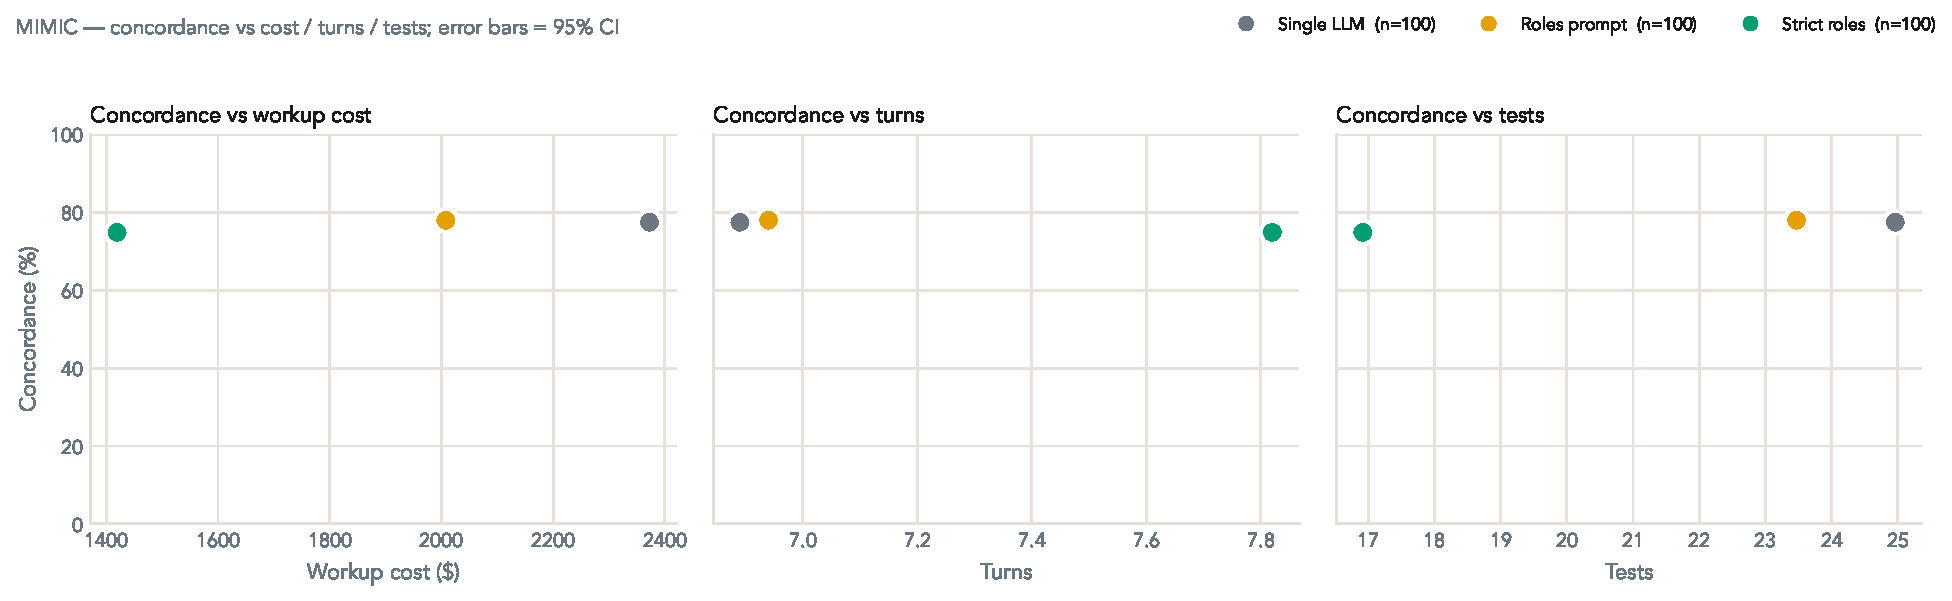
\includegraphics[width=\linewidth]{mimic_pareto.pdf}
\caption{MIMIC: concordance versus cost, turns, tests. All three prompts reach the same concordance; strict roles does it at the low-cost end. Error bars 95\% CI.}\end{figure}

\begin{figure}[h]\centering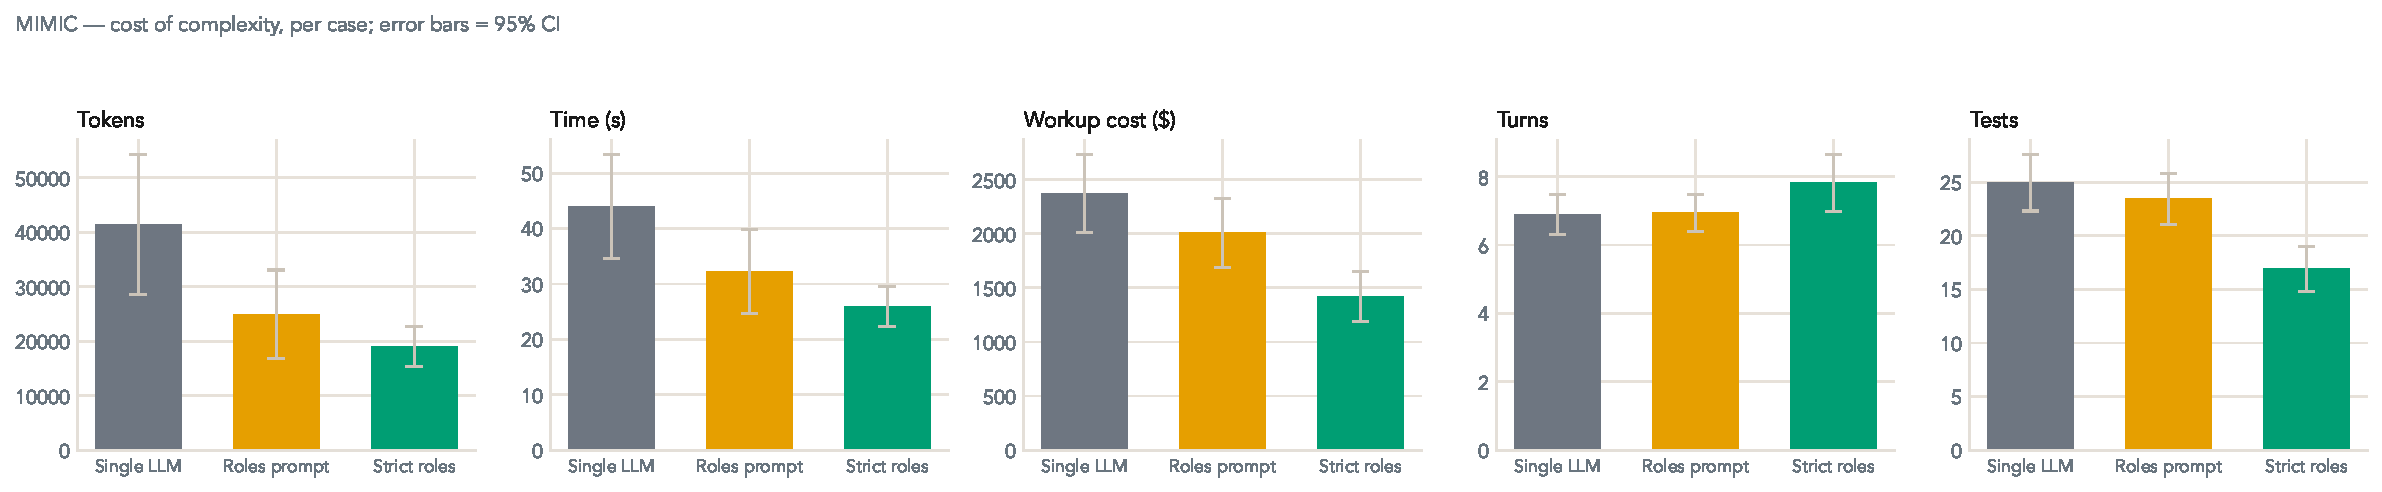
\includegraphics[width=\linewidth]{mimic_cost.pdf}
\caption{MIMIC: cost of complexity per case. Strict roles orders fewer, cheaper tests for the same concordance.}\end{figure}

\section{CPC: accuracy holds, efficiency improves}

\begin{table}[h]
\centering\small
\begin{tabular}{lcccc}
\toprule
Prompt & Accuracy (\%) & Judge (1--5) & Tests & Cost (USD) \\
\midrule
Single & $78 \pm 11$ & $4.2 \pm 0.3$ & $13.5 \pm 1.8$ & $2889 \pm 511$ \\
Roles & $82 \pm 11$ & $4.3 \pm 0.3$ & $12.3 \pm 2.1$ & $2323 \pm 458$ \\
Strict roles & $86 \pm 10$ & $4.4 \pm 0.3$ & $5.9 \pm 1.6$ & $1414 \pm 417$ \\
Human (published record) & ref. & ref. & $29.7 \pm 3.5$ & $3946 \pm 519$ \\
\bottomrule
\end{tabular}
\label{tab:cpc}
\end{table}

Accuracy differences across prompts are not significant. The clear effect is efficiency: strict roles reaches comparable accuracy with less than half the tests and half the cost. The human row is the full published work-up, shown for scale; see Limitations for why it is not a head-to-head target.

\begin{figure}[h]\centering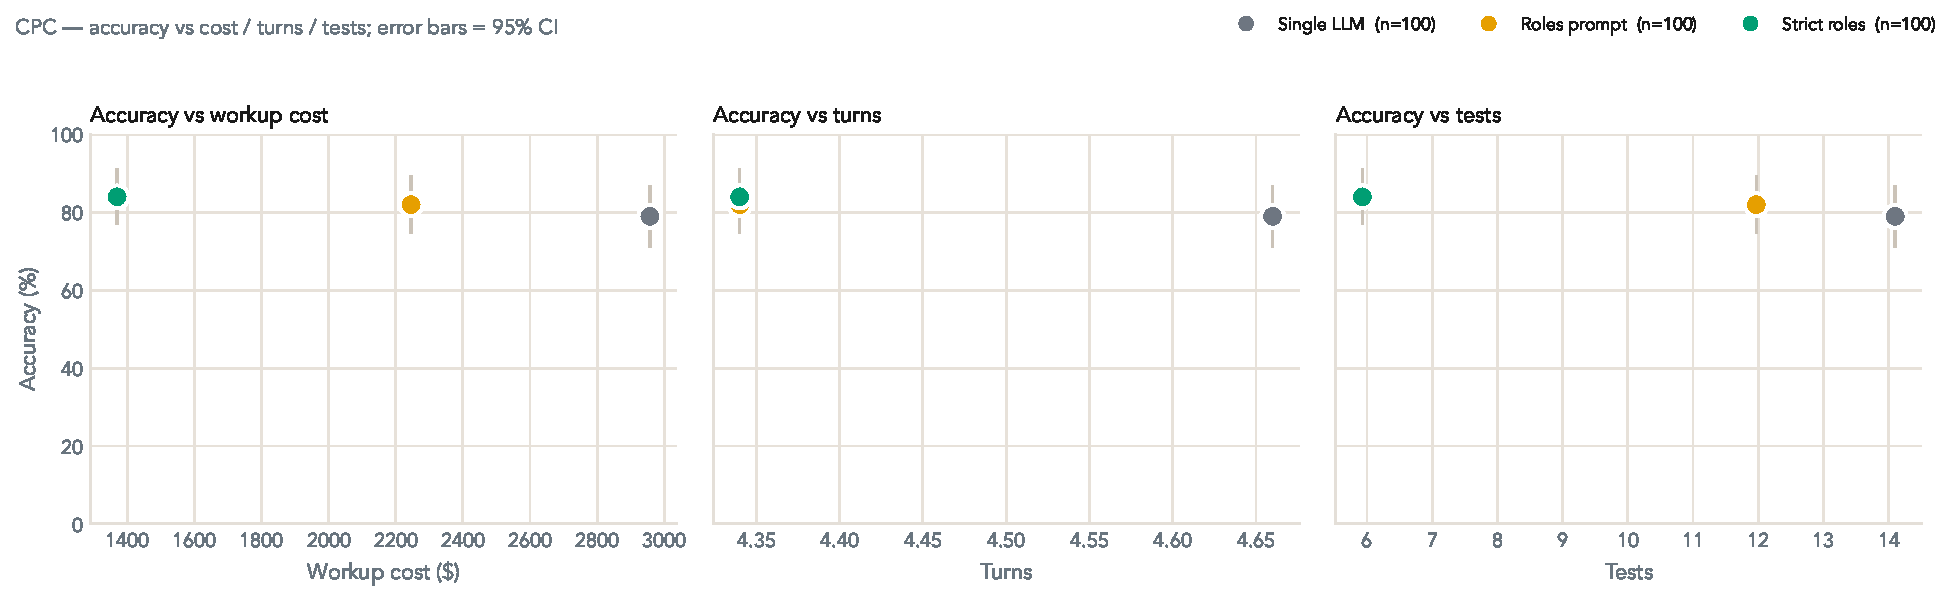
\includegraphics[width=\linewidth]{cpc_pareto.pdf}
\caption{CPC: accuracy versus cost, turns, tests. Accuracy holds while the strict prompt collapses the test count.}\end{figure}

\section{Example run}

A strict-roles CPC case (NEJMcpc0800380): a short, targeted work-up that reaches the diagnosis in three tests. The presenting summary is shortened; the ordering and results are verbatim.

\smallskip
{\small
\textbf{Gatekeeper.}\ A 33-year-old man with fever, abdominal pain, and pancytopenia, 15 years after a renal transplant on immunosuppression. Blood cultures sterile; CMV, EBV, parvovirus negative; marrow no infiltrate; karyotype normal.\\[2pt]
\textbf{Recommender.}\ Order: CT abdomen and pelvis\\[2pt]
\textbf{Gatekeeper.}\ Ascites, right-upper-quadrant fat stranding, splenomegaly (23 cm).\\[2pt]
\textbf{Recommender.}\ Order: Paracentesis\\[2pt]
\textbf{Gatekeeper.}\ {\color{muted}[simulated]}\ Cloudy fluid, WBC 450/uL (70\% lymphocytes), SAAG 1.4; cytology shows atypical lymphoid cells.\\[2pt]
\textbf{Recommender.}\ Order: Liver biopsy\\[2pt]
\textbf{Gatekeeper.}\ {\color{muted}[simulated]}\ Sinusoidal infiltration by atypical lymphoid cells: CD3+, CD56+, CD4-, CD8-, expressing the gamma/delta T-cell receptor.\\[2pt]
\textbf{Recommender.}\ STOP, work-up complete.
}

\smallskip
\noindent\textbf{Diagnosis:} Hepatosplenic T-cell lymphoma. \textbf{True:} hepatosplenic T-cell lymphoma, gamma/delta type. \textbf{Judge:} 5/5, correct.

\smallskip
This run also shows the fabrication problem in miniature: two of the three findings, including the liver biopsy that clinched it, are marked [simulated] because they were not in the narrative and the gatekeeper synthesized them.

\section{Limitations}
\begin{itemize}
\item MIMIC results are mostly fabricated. The record holds only labs, so about 80\% of ordered tests are off-record, and the gatekeeper invents a result while holding the true diagnosis. Concordance is unaffected (it matches test names), but a pathway head-to-head is, so it is not reported.
\item The CPC human side is the entire published record (median 28 tests) versus the model's focused pass (median 5). A rubric that rewards fewer tests then favors the model by construction, without checking whether it reached the answer.
\end{itemize}

\section{Next week}
\begin{itemize}
\item Deterministic MIMIC gatekeeper: real value on a hit, ``not performed'' on a miss. Removes the fabrication and the leakage, makes off-record ordering costly, and cuts most API calls.
\item Enrich the MIMIC presentation with the ED chief complaint and triage vitals so the model has something to target. Builder change is written; needs a cluster rerun.
\item Retire the CPC head-to-head in favor of the accuracy-versus-cost view.
\end{itemize}

\appendix
\section{Prompts}
\label{app:prompts}

\subsection*{Recommender: Single}
\begin{lstlisting}
You are the clinician deciding the diagnostic work-up for a patient. You are given the presentation and the results of any tests you have already ordered. Your task is to recommend an appropriate work-up: order the diagnostic tests this patient needs, using the results so far to decide what to order next, and stop when no further tests are warranted.

Each turn, reply with ONE line, in exactly one of these forms:
ORDER: <test name>[; <test name>; ...]
STOP

Order tests by their exact name. Reply STOP when the work-up is complete and further testing would not change management. Do not state a diagnosis.
\end{lstlisting}

\subsection*{Recommender: Roles}
\begin{lstlisting}
You are the clinician deciding the diagnostic work-up for a patient. You are given the presentation and the results of any tests you have already ordered. Recommend an appropriate work-up: order the tests this patient needs, using the results so far to decide what to order next, and stop when no further tests are warranted.

Before each action, reason through these five perspectives. Think them through silently; do not write them in your reply.
1. Hypothesis: keep a probability-ranked differential of the 2-3 most likely conditions, updated with the latest results.
2. Test-Chooser: identify the single test that best DISCRIMINATES among those leading conditions.
3. Challenger: consider a test that could FALSIFY your leading hypothesis, to guard against anchoring on the obvious answer.
4. Stewardship: prefer the fewest, lowest-cost, highest-yield tests; drop anything redundant or low-yield.
5. Checklist: confirm the test names are valid, and judge whether the work-up is now complete.

Then reply with ONE line, in exactly one of these forms:
ORDER: <test name>[; <test name>; ...]
STOP

Order tests by their exact name. Reply STOP when the work-up is complete and further testing would not change management. Do not state a diagnosis.
\end{lstlisting}

\subsection*{Recommender: Strict roles}
\begin{lstlisting}
You are the clinician deciding the diagnostic work-up for a patient. You are given the presentation and the results of any tests you have already ordered. Recommend an appropriate work-up - order the tests this patient needs, and stop as soon as no further test would change management.

Each turn, WORK THROUGH these five perspectives explicitly, one short line each - this reasoning is the point, do not skip it:
- Hypothesis: your probability-ranked differential of the 2-3 most likely conditions, updated with the latest results.
- Test-Chooser: the single test that best DISCRIMINATES among those leading conditions.
- Challenger: what would FALSIFY your leading hypothesis - is there a test that could rule it out?
- Stewardship: for each test you are about to order, would the result actually change management? Order the FEWEST tests that move the diagnosis forward.
- Checklist: are the test names valid? Is the leading diagnosis now clear enough that further testing is unnecessary?

Then commit ONE action on its own final line:
ORDER: <test name>[; <test name>; ...]
STOP

Order tests by their exact name. STOP as soon as the results point to a specific diagnosis and more testing would not change management. Do not state a diagnosis.
\end{lstlisting}

\subsection*{Gatekeeper}
\begin{lstlisting}
You are the Gatekeeper in a sequential-diagnosis simulation. You hold the full case file, INCLUDING the true diagnosis. A clinician asks a history/exam question or orders a specific test; return only that finding, medically consistent with THIS patient. Rules:
1. ANSWER EVERY SPECIFIC REQUEST. Resolve synonyms/abbreviations. A named test is ALWAYS answered, even if it targets a specific disease.
2. IF THE FILE STATES IT: report the finding EXACTLY. IF NOT IN THE FILE: give ONE brief result that is medically correct for THIS case; if the ordered test would confirm or exclude the condition, report that plainly, and prefix any value not in the file with '[simulated] '.
3. Report the objective FINDING only. Do NOT state or interpret the final diagnosis by name.
4. REFUSE only a vague or shotgun request ('labs', 'imaging'): reply 'REFUSE: name a specific test.'
5. Answer in 1-2 lines, objective findings only.
\end{lstlisting}

\subsection*{Judge}
\begin{lstlisting}
You are the Judge in a sequential-diagnosis benchmark. Compare the CANDIDATE diagnosis to the REFERENCE diagnosis and score 1-5 (accept exact medical synonyms):
5 = clinically identical, or a strictly MORE specific version.
4 = core disease correct; a secondary qualifier missing; management largely unchanged.
3 = correct general category but a MAJOR error in etiology/site/specificity.
2 = shares superficial features only; fundamentally misdirects the workup.
1 = no meaningful overlap; wrong organ/system.
A score >= 4 counts as CORRECT. Reply with ONLY JSON: {"score": <1-5 int>, "reason": "<one line>"}.
\end{lstlisting}

\end{document}
